\subsection{The SIR model}
\label{sec:sir_model}

The \textit{explanatory} SIR model is a very well studied and understood compartment model from epidemiology \cite{kermack_contribution_1927}, which allows to simulate the dynamics of an infectious disease like influenza, tuberculosis, chicken pox, rubella and measles spreading through a population.

In this model, people in a population of size $N$ can be in either one of the three states \textit{Susceptible}, \textit{Infected} or \textit{Recovered} at a particular time, where it is assumed that initially there is at least one infected person in the population. People interact \textit{on average} with a given rate of $\beta$ other people per time-unit and become infected with a given probability $\gamma$ when interacting with an infected person. When infected, a person recovers \textit{on average} after $\delta$ time-units and is then immune to further infections. An interaction between infected persons does not lead to re-infection, thus these interactions are ignored in this model. This definition gives rise to three compartments with the transitions seen in Figure \ref{fig:sir_transitions}.

\begin{figure}
	\centering
	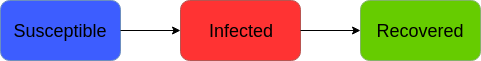
\includegraphics[width=.7\textwidth, angle=0]{./fig/timedriven/SIR_transitions.png}
	\caption{States and transitions in the SIR compartment model.}
	\label{fig:sir_transitions}
\end{figure}

This model was also formalized using System Dynamics (SD) \cite{porter_industrial_1962}. In SD one models a system through differential equations, allowing to conveniently express continuous systems, which change over time, solving them by numerically integrating over time, which gives then rise to the dynamics. The SIR model is modelled using the following equation, with the dynamics shown in Figure \ref{fig:sir_sd_dynamics} .

\begin{equation}
\begin{aligned}
\frac{\mathrm d S}{\mathrm d t} = -infectionRate \\
\frac{\mathrm d I}{\mathrm d t} = infectionRate - recoveryRate \\
\frac{\mathrm d R}{\mathrm d t} = recoveryRate 
\end{aligned}
\end{equation}

\begin{equation}
\begin{aligned}
infectionRate = \frac{I \beta S \gamma}{N} \\
recoveryRate = \frac{I}{\delta} 
\end{aligned}
\end{equation}

\begin{figure}
	\centering
	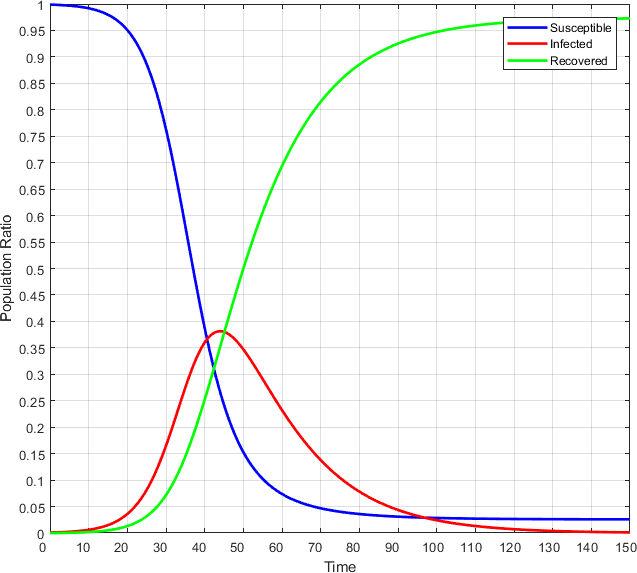
\includegraphics[width=0.5\textwidth, angle=0]{./fig/timedriven/SIR_SD_1000agents_150t_001dt.png}
	\caption{Dynamics of the SIR compartment model using the System Dynamics approach. Population Size $N$ = 1,000, contact rate $\beta =  \frac{1}{5}$, infection probability $\gamma = 0.05$, illness duration $\delta = 15$ with initially 1 infected agent. Simulation run for 150 time steps. Generated using our pure functional SD approach (see Appendix \ref{app:sd_simulation}).}
	\label{fig:sir_sd_dynamics}
\end{figure}

The approach of mapping the SIR model to an ABS is to discretize the population and model each person in the population as an individual agent. The transitions between the states are happening due to discrete events caused both by interactions amongst the agents and timeouts. The major advantage of ABS over SD is that it allows to incorporate spatiality and simulate heterogeneity of population e.g. different sex, age. This is not directly possible with other simulation methods of SD or Discrete Event Simulation (DES) \cite{zeigler_theory_2000}.

In the ABS classification of \cite{macal_everything_2016}, this model can be seen as an \textit{Interactive ABMS}: agents are individual heterogeneous agents with diverse set characteristics; they have autonomic, dynamic, endogenously defined behaviour; interactions happen between other agents and the environment through observed states and behaviours of other agents and the state of the environment.